\documentclass[tikz,border=2cm]{standalone}
\usetikzlibrary{shapes.geometric, arrows.meta}

\begin{document}

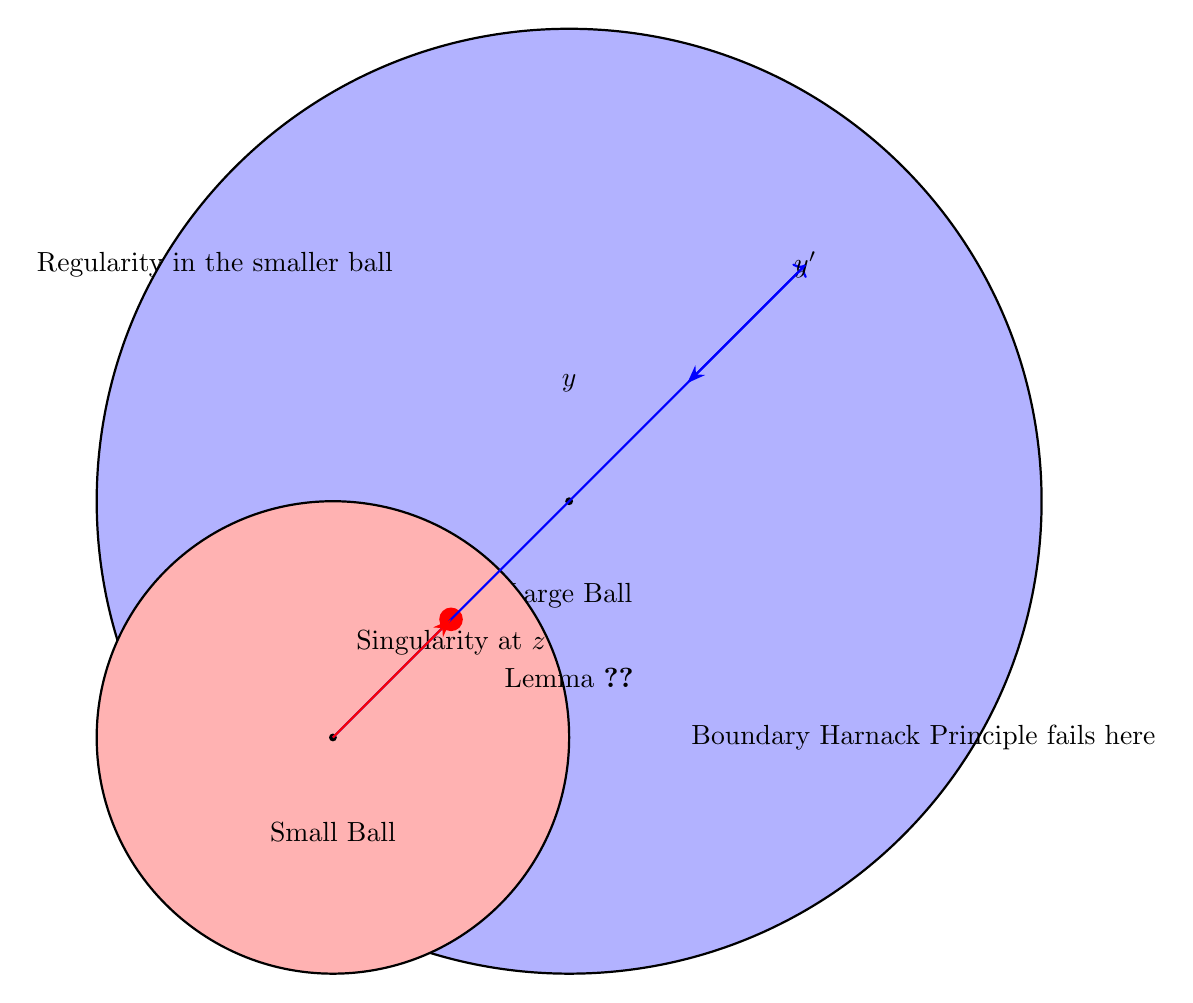
\begin{tikzpicture}[scale=1.5]

% Draw the large ball
\draw[thick, fill=blue!30] (0,0) circle (4);
\node at (0,0) [circle, inner sep=1pt, fill=black] (centerL) {};
\node at (0,-0.8) {Large Ball};

% Draw the small ball
\draw[thick, fill=red!30] (-2,-2) circle (2);
\node at (-2,-2) [circle, inner sep=1pt, fill=black] (centerS) {};
\node at (-2,-2.8) {Small Ball};

% Draw the singularity
\fill[red] (-1,-1) circle (0.1);
\node at (-1,-1.2) {Singularity at $z$};

% Draw the line segment from y to y'
\draw[->, thick, blue] (-2,-2) -- (2,2);
\node at (0,1) {$y$};
\node at (2,2) {$y'$};

% Draw the arrows indicating the boundaries
\draw[-Stealth, thick, red] (-2,-2) -- (-1,-1);
\draw[-Stealth, thick, blue] (2,2) -- (1,1);

% Add labels
\node at (0,-1.5) {Lemma~\ref{lem:gdint}};
\node at (-3,2) {Regularity in the smaller ball};
\node at (3,-2) {Boundary Harnack Principle fails here};

\end{tikzpicture}

\end{document}